\documentclass{fkssolpub}

\usepackage[czech]{babel}
\usepackage{fontspec}
\usepackage{fkssugar}
\usepackage{amsmath}
\usepackage{graphicx}
\usepackage{wrapfig}
\usepackage{subcaption}

\author{Ondřej Sedláček}
\school{Gymnázium Oty Pavla} 
\series{FO-B-S}
\problem{6} 

\begin{document} 

Pro analýzu pádu jsem použil kuličku o hmotnosti 2 g, kuličku o hmotnosti
35 g a video s 60 fps. Pád jsem měřil na vzdálenost 2,5 metru. Naměřené
hodnoty pro lehčí kuličku najdeme v tabulce \ref{tab:b} a pro těžší v
tabulce \ref{tab:c}.

Fitováním metodou nejmenších čtverců nám pro odporovou sílu působící
na lehkou kuličku vyjde funkce:

\[
	F_{ol}(v) = 0{,}000318 \cdot v^{2{,}074}
\]

Pro těžkou kuličku nám vyjde funkce:

\[
	F_{ot}(v) = 0{,}000326 \cdot v^{2{,}03905}
\]

Obě měli koeficient determinace kolem 99{,}9 \%, tudíž tato funkce
přesně reprezentuje experimentální data. Můžeme si všimnout, že obě
odporové síli se příliš neliší, tudíž můžeme usoudit, že velikost
odporové síli nezávisí na hmotnosti. To způsobí, že na těžký předmět
bude mít odporová síla malý efekt, ale na lehký předmět výrazný (to
můžeme vidět na grafech níže). Z toho tedy vyvodíme, že u hustých předmětů
lze odporová síla při volném pádu zanedbat.

\begin{figure}[h!]
	\caption{Grafy}
	\begin{subfigure}[b]{0.5\textwidth}
		\centering
		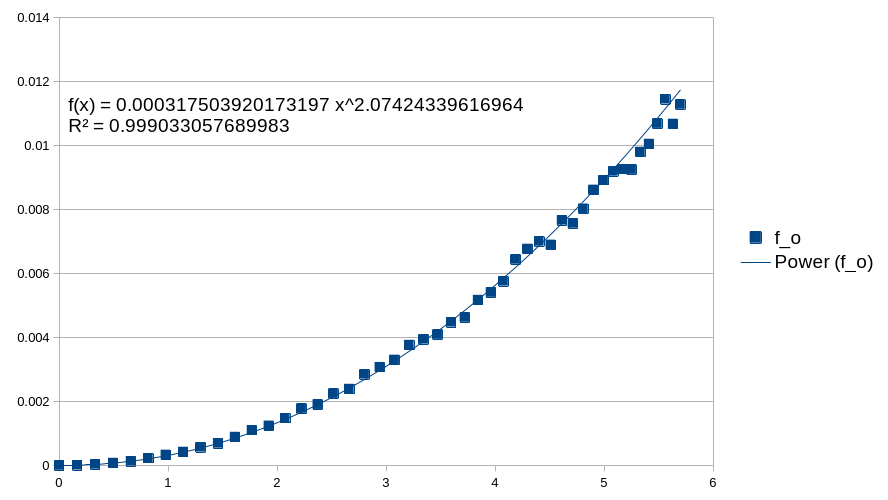
\includegraphics[width=\textwidth]{6-fig1.png}
		\caption{Odporová síla $F_o$ s lehkou kuličkou}
		\label{fig:a}
	\end{subfigure}
	\begin{subfigure}[b]{0.5\textwidth}
		\centering
		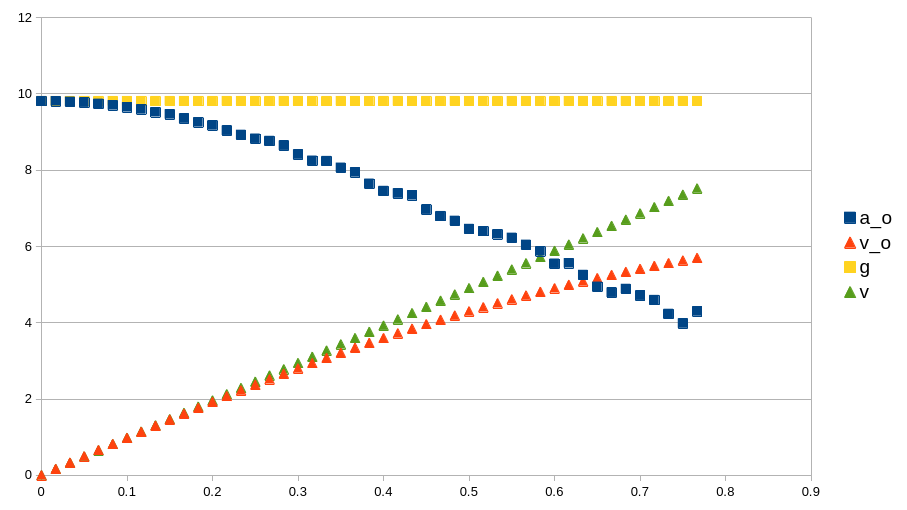
\includegraphics[width=\textwidth]{6-fig2.png}
		\caption{Dráha a porovnání zrychlení a rychlosti s odporem a bez odporu (lehká kulička)}
		\label{fig:b}
	\end{subfigure}
	\begin{subfigure}[b]{0.5\textwidth}
		\centering
		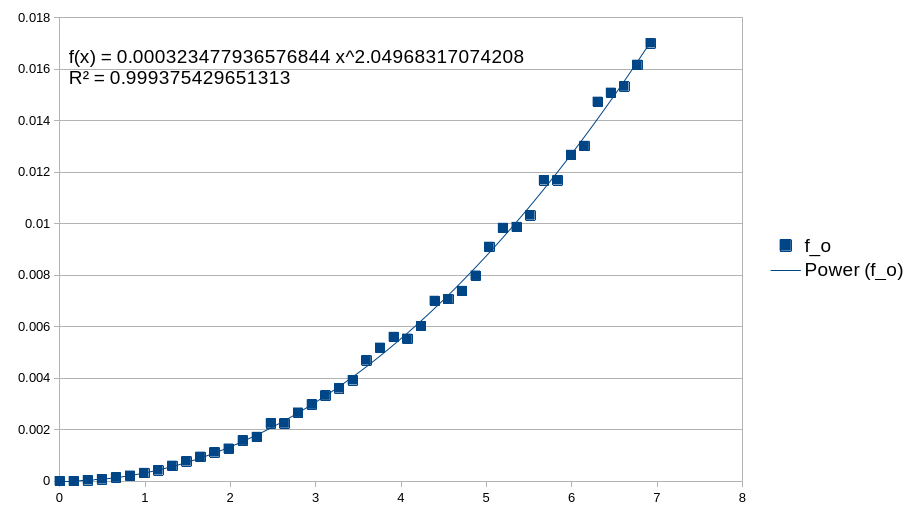
\includegraphics[width=\textwidth]{6-fig3.png}
		\caption{Odporová síla $F_o$ s těžkou kuličkou}
		\label{fig:c}
	\end{subfigure}
	\begin{subfigure}[b]{0.5\textwidth}
		\centering
		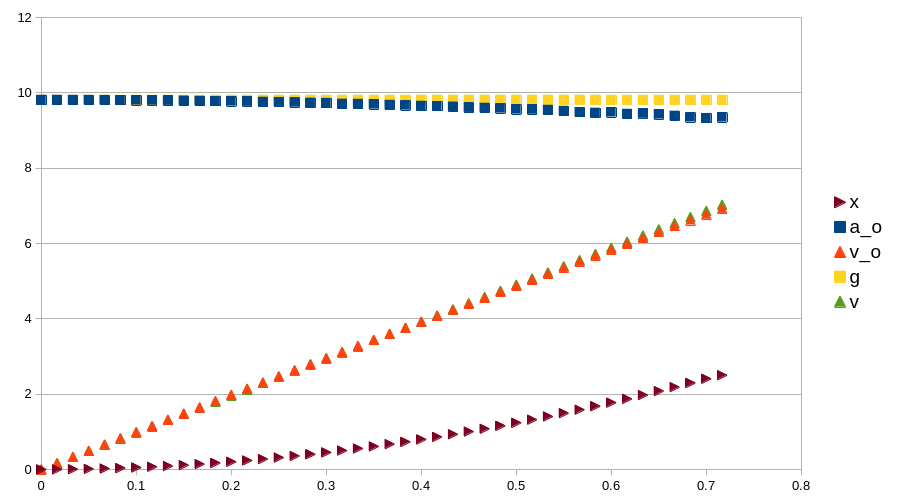
\includegraphics[width=\textwidth]{6-fig4.png}
		\caption{Dráha a porovnání zrychlení a rychlosti s odporem a bez odporu (těžká kulička)}
		\label{fig:d}
	\end{subfigure}
\end{figure}

\begin{table}[h!]
	\caption{Výsledky měření}
	\begin{subtable}[c]{0.5\textwidth}
		\subcaption{Výsledky měření s lehkou kuličkou}
		\label{tab:b}
		% \begin{center}
		\begin{tabular}{|c|c|c|c|c|}
			\hline
			$t$ & $s$ [m] & $v$ [m/s] & $a$ [m$\cdot$s$^{-2}$]& $F_o$ [N] \\
			\hline
0 & 0 & 0 & 9,81 & 0 \\
0,01667 & 0,001 & 0,165 & 9,807 & 0,000006 \\
0,03333 & 0,006 & 0,33 & 9,794 & 0,000032 \\
0,05 & 0,013 & 0,495 & 9,771 & 0,000078 \\
0,06667 & 0,023 & 0,658 & 9,744 & 0,000132 \\
0,08333 & 0,036 & 0,818 & 9,696 & 0,000228 \\
0,1 & 0,051 & 0,978 & 9,644 & 0,000332 \\
0,11667 & 0,069 & 1,138 & 9,598 & 0,000424 \\
0,13333 & 0,089 & 1,298 & 9,526 & 0,000568 \\
0,15 & 0,113 & 1,458 & 9,465 & 0,00069 \\
0,16667 & 0,138 & 1,613 & 9,365 & 0,00089 \\
0,18333 & 0,167 & 1,768 & 9,259 & 0,001102 \\
0,2 & 0,197 & 1,923 & 9,19 & 0,00124 \\
0,21667 & 0,232 & 2,074 & 9,071 & 0,001478 \\
0,23333 & 0,267 & 2,224 & 8,921 & 0,001778 \\
0,25 & 0,307 & 2,374 & 8,86 & 0,0019 \\
0,26667 & 0,347 & 2,519 & 8,687 & 0,002246 \\
0,28333 & 0,391 & 2,664 & 8,615 & 0,00239 \\
0,3 & 0,436 & 2,805 & 8,386 & 0,002848 \\
0,31667 & 0,485 & 2,945 & 8,274 & 0,003072 \\
0,33333 & 0,535 & 3,081 & 8,16 & 0,0033 \\
0,35 & 0,588 & 3,215 & 7,928 & 0,003764 \\
0,36667 & 0,643 & 3,348 & 7,839 & 0,003942 \\
0,38333 & 0,7 & 3,478 & 7,765 & 0,00409 \\
0,4 & 0,76 & 3,603 & 7,573 & 0,004474 \\
0,41667 & 0,82 & 3,728 & 7,498 & 0,004624 \\
0,43333 & 0,885 & 3,849 & 7,225 & 0,00517 \\
0,45 & 0,95 & 3,969 & 7,108 & 0,005404 \\
0,46667 & 1,017 & 4,086 & 6,933 & 0,005754 \\
0,48333 & 1,087 & 4,199 & 6,591 & 0,006438 \\
0,5 & 1,157 & 4,308 & 6,426 & 0,006768 \\
0,51667 & 1,231 & 4,416 & 6,308 & 0,007004 \\
0,53333 & 1,306 & 4,521 & 6,362 & 0,006896 \\
0,55 & 1,381 & 4,622 & 5,98 & 0,00766 \\
0,56667 & 1,46 & 4,722 & 6,028 & 0,007564 \\
0,58333 & 1,54 & 4,818 & 5,798 & 0,008024 \\
0,6 & 1,62 & 4,91 & 5,503 & 0,008614 \\
0,61667 & 1,703 & 5,001 & 5,353 & 0,008914 \\
0,63333 & 1,788 & 5,088 & 5,215 & 0,00919 \\
0,65 & 1,873 & 5,173 & 5,18 & 0,00926 \\
0,66667 & 1,959 & 5,256 & 5,187 & 0,009246 \\
0,68333 & 2,049 & 5,337 & 4,911 & 0,009798 \\
0,7 & 2,139 & 5,416 & 4,786 & 0,010048 \\
0,71667 & 2,229 & 5,493 & 4,468 & 0,010684 \\
0,73333 & 2,321 & 5,566 & 4,088 & 0,011444 \\
0,75 & 2,416 & 5,639 & 4,473 & 0,010674 \\
0,76667 & 2,5 & 5,706 & 4,17 & 0,01128 \\
			\hline
		\end{tabular}
		% \end{center}

	\end{subtable}
	\begin{subtable}[c]{0.5\textwidth}
		\subcaption{Výsledky měření s těžkou kuličkou}
		\label{tab:c}
		\begin{tabular}{|c|c|c|c|c|}
			\hline
			$t$ & $s$ [m] & $v$ [m/s] & $a$ [m$\cdot$s$^{-2}$]& $F_o$ [N] \\
			\hline
0 & 0 & 0 & 9,81 & 0 \\
0,01667 & 0,001 & 0,165 & 9,81 & 0 \\
0,03333 & 0,006 & 0,33 & 9,809 & 0,000035 \\
0,05 & 0,013 & 0,495 & 9,808 & 0,00007 \\
0,06667 & 0,023 & 0,66 & 9,806 & 0,00014 \\
0,08333 & 0,036 & 0,825 & 9,804 & 0,00021 \\
0,1 & 0,051 & 0,99 & 9,801 & 0,000315 \\
0,11667 & 0,07 & 1,155 & 9,798 & 0,00042 \\
0,13333 & 0,09 & 1,32 & 9,793 & 0,000595 \\
0,15 & 0,115 & 1,485 & 9,788 & 0,00077 \\
0,16667 & 0,141 & 1,65 & 9,783 & 0,000945 \\
0,18333 & 0,171 & 1,815 & 9,778 & 0,00112 \\
0,2 & 0,202 & 1,98 & 9,774 & 0,00126 \\
0,21667 & 0,237 & 2,145 & 9,765 & 0,001575 \\
0,23333 & 0,274 & 2,31 & 9,761 & 0,001715 \\
0,25 & 0,314 & 2,474 & 9,746 & 0,00224 \\
0,26667 & 0,357 & 2,634 & 9,746 & 0,00224 \\
0,28333 & 0,402 & 2,794 & 9,734 & 0,00266 \\
0,3 & 0,451 & 2,954 & 9,725 & 0,002975 \\
0,31667 & 0,501 & 3,114 & 9,715 & 0,003325 \\
0,33333 & 0,555 & 3,274 & 9,707 & 0,003605 \\
0,35 & 0,61 & 3,434 & 9,698 & 0,00392 \\
0,36667 & 0,67 & 3,594 & 9,676 & 0,00469 \\
0,38333 & 0,731 & 3,754 & 9,662 & 0,00518 \\
0,4 & 0,796 & 3,914 & 9,65 & 0,0056 \\
0,41667 & 0,862 & 4,074 & 9,652 & 0,00553 \\
0,43333 & 0,932 & 4,234 & 9,638 & 0,00602 \\
0,45 & 1,004 & 4,394 & 9,61 & 0,007 \\
0,46667 & 1,079 & 4,554 & 9,608 & 0,00707 \\
0,48333 & 1,157 & 4,714 & 9,599 & 0,007385 \\
0,5 & 1,237 & 4,874 & 9,582 & 0,00798 \\
0,51667 & 1,32 & 5,034 & 9,55 & 0,0091 \\
0,53333 & 1,405 & 5,194 & 9,529 & 0,009835 \\
0,55 & 1,494 & 5,354 & 9,528 & 0,00987 \\
0,56667 & 1,584 & 5,514 & 9,515 & 0,010325 \\
0,58333 & 1,678 & 5,674 & 9,476 & 0,01169 \\
0,6 & 1,773 & 5,834 & 9,476 & 0,01169 \\
0,61667 & 1,873 & 5,993 & 9,448 & 0,01267 \\
0,63333 & 1,974 & 6,15 & 9,438 & 0,01302 \\
0,65 & 2,079 & 6,305 & 9,389 & 0,014735 \\
0,66667 & 2,185 & 6,46 & 9,379 & 0,015085 \\
0,68333 & 2,295 & 6,615 & 9,372 & 0,01533 \\
0,7 & 2,406 & 6,77 & 9,348 & 0,01617 \\
0,71667 & 2,5 & 6,925 & 9,324 & 0,01701 \\
			\hline
		\end{tabular}

	\end{subtable}
\end{table}

\end{document}
